Based on  autocorrelations\only<1>{\footnote{Broto, P., Moreau, G. and Vandycke, C. \textit{Eur. J. Med. Chem.}, 19(1):71-78, 1984.}}\only<2->{\setcounter{footnote}{3} and modified for TMCs}\only<2->{\footnote{Janet, J.P., and Kulik, H.J. \textit{J. Phys. Chem. A}, 2017,121, 46, 8939-8954.}}

\begin{tikzpicture}[node distance=20pt]
\tikzstyle{boxes}=[draw=red, rounded corners]
\definecolor{dist}{rgb}{0,0,0.54}
\definecolor{prox}{rgb}{0.6953125,0.1328125,0.1325125}
\definecolor{mid}{rgb}{0,0.39,0}
\tikzstyle{met} = [circle, draw, fill=blue!20,minimum size = 1.5cm, 
text width=1.25cm, text badly centered, node distance=3cm, inner sep=0pt]
\tikzstyle{graphn} = [circle, draw, thick, fill=darkgray!20,minimum size = 0.5cm, 
text width=1cm, text badly centered, node distance=3cm, inner sep=0pt]
\tikzstyle{carb} = [circle, draw, fill=gray!20,minimum size = 1cm, 
text width=1cm, text badly centered, node distance=3cm, inner sep=0pt]
\tikzstyle{ox} = [circle, draw, fill=red!20,minimum size = 0.5cm, 
text width=0.8cm, text badly centered, node distance=3cm, inner sep=0pt]  

\visible<14->{\fill[fill=dist!45]
    (-2,3) -- (-2,-2)  -- (2,-2) --(2,3);}
\visible<14->{\fill[fill=mid!45]
    (-2,3) -- (-2,-0.75)  -- (2,-0.75) --(2,3);}
\visible<14->{\fill[fill=prox!45]
    (-2,3) -- (-2,0.75)  -- (2,0.75) --(2,3);}
%%%%%%%%%%%%%%%%%%%%%%%%%%%%%%%%%%%%%5
\visible<1-17>{\node[ox] at (1.5,1.5) (ox1){O};}
\visible<1-17>{\node[ox] at (-1.5,1.5) (ox2){O};}
\visible<1-17>{\node[ox] at (1.5,-1.5) (ox3){O};}
\visible<1-17>{\node[ox] at (-1.5,-1.5) (ox4){O};}
\visible<1-17>{\node[carb] at (-0.75,0) (c1){C};}
\visible<1-17>{\node[carb] at (0.75,0) (c2){C};}
\visible<8-17>{\node[met] at (0,3) (m){M};}
\visible<1-17>{\path[draw, very thick] (ox1) -- (c2){};}
\visible<1-17>{\path[draw, very thick] (ox2) -- (c1){};}
\visible<1-17>{\path[draw, very thick] (ox3) -- (c2){};}
\visible<1-17>{\path[draw, very thick] (ox4) -- (c1){};}
\visible<1-17>{\path[draw, very thick] (c2) -- (c1){};}
\visible<1-17>{\path[draw, very thick] (c2) -- (c1){};}
\visible<8-17>{\path[draw,dashed, very thick] (m) -- (ox1){};}
\visible<8-17>{\path[draw,dashed, very thick] (m) -- (ox2){};}

%%%%%%%%%%%%%%%%%%%%%%%%%%%%%%%%%%%%%5 
\visible<2-4>{\node[fill  = orange!50,draw = red, ultra thick, fill opacity = 0.15,rounded corners,rectangle,minimum size=1.25cm] at (ox2.center){};}
\visible<3-4>{\node[fill  = blue!50,draw = blue,dashed, ultra thick, fill opacity = 0.05,rounded corners,rectangle,minimum size=1.05cm,rotate = 45] at (c1.center){};}
\visible<3-4>{\path[draw, ultra thick] (ox2.center) edge[bend left,blue,->] (c1.center);}
\visible<4>{\node[anchor = west] (eq) at (2.0,1.5){\small $\begin{aligned} \color{blue}d_1\color{black} : \sum_{\color{red}{O}\color{black},\color{gray}{C}}\color{black} Z_{O}Z_{C} = 48\end {aligned}$};}

\visible<5>{\node[fill  = orange!50,draw = red, ultra thick, fill opacity = 0.15,rounded corners,rectangle,minimum size=1.25cm] at (c1.center){};}
\visible<5>{\node[fill  = blue!50,draw = blue,dashed, ultra thick, fill opacity = 0.05,rounded corners,rectangle,minimum size=1.05cm,rotate = 45] at (ox2.center){};}
\visible<5>{\node[fill  = blue!50,draw = blue,dashed, ultra thick, fill opacity = 0.05,rounded corners,rectangle,minimum size=1.05cm,rotate = 45] at (ox4.center){};}
\visible<5>{\node[fill  = blue!50,draw = blue,dashed, ultra thick, fill opacity = 0.05,rounded corners,rectangle,minimum size=1.05cm,rotate = 45] at (c2.center){};}
\visible<5>{\node[anchor = west] (eq) at (2.0,1.5){\small $\begin{aligned} \color{blue}d_1\color{black} : 48 +  \sum_{\color{gray}{C}\color{black},\color{red}{O}}\color{black} Z_{O}Z_{C} = 144 + 48\end {aligned}$};}
\visible<5>{\path[draw, ultra thick] (c1.center) edge[bend left,blue,->] (c2.center);}
\visible<5>{\path[draw, ultra thick] (c1.center) edge[bend left,blue,->] (ox2.center);}
\visible<5>{\path[draw, ultra thick] (c1.center) edge[bend right,blue,->] (ox4.center);}


\visible<6>{\node[fill  = orange!50,draw = red, ultra thick, fill opacity = 0.15,rounded corners,rectangle,minimum size=1.25cm] at (c1.center){};}
\visible<6>{\node[fill  = orange!50,draw = red, ultra thick, fill opacity = 0.15,rounded corners,rectangle,minimum size=1.25cm] at (c2.center){};}
\visible<6>{\node[fill  = orange!50,draw = red, ultra thick, fill opacity = 0.15,rounded corners,rectangle,minimum size=1.25cm] at (ox1.center){};}
\visible<6>{\node[fill  = orange!50,draw = red, ultra thick, fill opacity = 0.15,rounded corners,rectangle,minimum size=1.25cm] at (ox2.center){};}
\visible<6>{\node[fill  = orange!50,draw = red, ultra thick, fill opacity = 0.15,rounded corners,rectangle,minimum size=1.25cm] at (ox3.center){};}
\visible<6>{\node[fill  = orange!50,draw = red, ultra thick, fill opacity = 0.15,rounded corners,rectangle,minimum size=1.25cm] at (ox4.center){};}
\visible<6>{\node[anchor = west] (eq) at (2.15,1.5){\small $\begin{aligned} \color{blue}d_1\color{black} : \sum_{i}\sum_{j}\color{black} Z_{i}Z_{j} \delta (d_{i,j},\color{blue}1\color{black}) \end {aligned}$};}
\visible<7>{\node[anchor = west] (eq) at (2.15,1.5){\small $\begin{aligned} \color{blue}d_x\color{black} : \sum_{i}\sum_{j}\color{black} Z_{i}Z_{j} \delta (d_{ij},\color{blue}x\color{black}) \end {aligned}$};}



%%%%%%%%%%%%%%%%%%%%%%%%%%%%%%%%%%%%%%%%%
%%%%%%%%%%%%%%%%%%%%%%%%%%%%%%%%%%%%%%%%%


\visible<7>{\node[anchor = west] (eq) at (2.15,-0.5){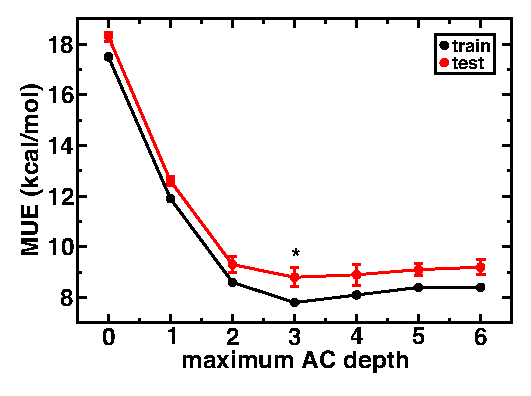
\includegraphics[width= 5.25cm]{representations/figures/ACD}};}


%%%%%%%%%%%%%%%%%%%%%%%%%%%%%%%%%%%%%%%%%
\visible<8->{\node[anchor = west] (eq) at (2.15,1.5){\small How to adapt to TM complexes?};}
\visible<9->{\node[anchor = west,align = left] (eq) at (2.15,0.80){\small restrict the scope to focus on \\ \small \textit{near-metal atoms}};}
%%%%%%%%%%%%%%%%%%%%%%%%%%%%%%%%%%%%%%%%%
\visible<10-12>{\node[fill  = orange!50,draw = red, ultra thick, fill opacity = 0.15,rounded corners,rectangle,minimum size=1.25cm] at (m.center){};}
\visible<11>{\node[fill  = blue!50,draw = blue,dashed, ultra thick, fill opacity = 0.05,rounded corners,rectangle,minimum size=1.05cm,rotate = 45] at (ox1.center){};}
\visible<11>{\node[fill  = blue!50,draw = blue,dashed, ultra thick, fill opacity = 0.05,rounded corners,rectangle,minimum size=1.05cm,rotate = 45] at (ox2.center){};}

\visible<11>{\path[draw, ultra thick,blue] (ox1.center) edge [bend right,<-] node {} (m.center){};}
\visible<11>{\path[draw, ultra thick,blue] (ox2.center) edge [bend left,<-] node {} (m.center){};}

\visible<11>{\node[anchor = west] (eq) at (2.0,-0.25){\small $\begin{aligned} \color{blue}d_1\color{black} : \sum_{\color{blue!50}{M}\color{black},\color{red}{O}} Z_{M}Z_O \end{aligned}$};}
%\visible<16>{\node[rectangle,minimum width = 1cm,black] (vectc1) at (-3,2){112};}

\visible<12>{\node[fill  = blue!50,draw = blue,dashed, ultra thick, fill opacity = 0.05,rounded corners,rectangle,minimum size=1.05cm,rotate = 45] at (c1.center){};}
\visible<12>{\node[fill  = blue!50,draw = blue,dashed, ultra thick, fill opacity = 0.05,rounded corners,rectangle,minimum size=1.05cm,rotate = 45] at (c2.center){};}

\visible<12>{\path[draw, ultra thick,blue] (c1.center) edge [bend left,<-] node {} (m.center){};}
\visible<12>{\path[draw, ultra thick,blue] (c2.center) edge [bend right,<-] node {} (m.center){};}

\visible<12>{\node[anchor = west] (eq) at (2.0,-0.25){\small $\begin{aligned} \color{blue}d_2\color{black} : \sum_{\color{blue!50}{M}\color{black},\color{gray}{C}} Z_{M}Z_C  \end{aligned}$};}


%%%%%%%%%%%%%%%%%%%%%%%%%%%%%%%55

\visible<13>{\node[fill  = blue!50,draw = blue,dashed, ultra thick, fill opacity = 0.05,rounded corners,rectangle,minimum size=1.05cm,rotate = 45] at (ox3.center){};}
\visible<13>{\node[fill  = blue!50,draw = blue,dashed, ultra thick, fill opacity = 0.05,rounded corners,rectangle,minimum size=1.05cm,rotate = 45] at (ox4.center){};}

\visible<13>{\path[draw, ultra thick,blue] (ox3.center) edge [bend right,<-] node {} (m.center){};}
\visible<13>{\path[draw, ultra thick,blue] (ox4.center) edge [bend left,<-] node {} (m.center){};}

\visible<13->{\node[anchor = west] (eq) at (2.0,-0.25){\small $\begin{aligned} \color{blue}d_3\color{black} : \sum_{\color{blue!50}{M}\color{black},\color{red}{O}} Z_{M}Z_O  \end{aligned}$};}






%%%%%%%%%%%%%%%%%%%%%%%%%%%%%%%%%%%%%%%%%
%\visible<13->{\node[fill  = orange!50,draw = red, ultra thick, fill opacity = 0.15,rounded corners,rectangle,minimum size=1.25cm] at (ox1.center){};}
%\visible<13->{\node[fill  = orange!50,draw = red, ultra thick, fill opacity = 0.15,rounded corners,rectangle,minimum size=1.25cm] at (ox2.center){};}
%
%\visible<13->{\node[anchor = west] (eq) at (2,-0.15){\small $\begin{aligned} \color{blue}d
%\color{black} : \frac{1}{\left\vert lc \right\vert}\sum_{i\in lc}\sum_{j} Z_iZ_j \delta (d_{ij}, 
%\color{blue}d\color{black}) \end{aligned}$};}%%


\visible<15->{\node[anchor = west,red, ultra thick] (neq) at (3,-1) {$
\color{red}\left(Z_i - Z_j\right)\color{black} $};}
\visible<16>{\node[anchor = west,rectangle,ultra thick] (neq) at (3,-1.75) {properties:$\color{black}T\color{black}$,$\color{black}\chi\color{black}$,$\color{black}Z\color{black}$,$\color{black}I\color{black}$,$\color{black}S\color{black}$ };}
\visible<17->{\node[anchor = west,rectangle,draw, ultra thick] (neq) at (4,-1.75) {\small $\sim 160$ features in total};}


%%%%%%%%%%%%%%%%%%%%%%%%%%%%%%%%%%%%%%%%%
\end{tikzpicture}